\documentclass[12pt,a4paper]{article}
\usepackage[utf8]{inputenc}
\usepackage[T1]{fontenc}
\usepackage[portuguese]{babel}
\usepackage{lmodern}
\usepackage[a4paper,margin=3cm]{geometry}
\usepackage{graphicx}
\usepackage{subcaption}
\usepackage{booktabs}
\usepackage{amsmath}
\usepackage{float}
\usepackage{enumitem}
\usepackage{fancyhdr}
\usepackage{xcolor}
\usepackage[colorlinks=true,urlcolor=blue,linkcolor=black]{hyperref}

\graphicspath{{../pictures/}}
\setlength{\parindent}{0pt}
\setlength{\parskip}{0.7em}
\pagestyle{fancy}
\fancyhf{}
\lhead{Departamento de Ciência de Computadores, FCUP}
\rhead{Inteligência Artificial CC2006}
\cfoot{\thepage}

\emergencystretch=3em
\newcommand{\code}[1]{\texttt{#1}}

\begin{document}

\begin{center}
  {\LARGE\bfseries Segundo Trabalho de Inteligência Artificial CC2006}\\[0.8em]
  {\large Classificação de dados de \emph{speed dating} com Árvores de Decisão e Naive Bayes}\\[1.2em]
  Pedro Miguel Ribeiro Carvalho, up201805068\\
  João Paulo Macedo Sampaio, up201805112\\[0.6em]
  Departamento de Ciência de Computadores, Faculdade de Ciências da Universidade do Porto\\
  Versão revista, \today
\end{center}

\begin{abstract}
\noindent
Machine Learning permite inferir padrões a partir de dados. Neste trabalho usámos dois algoritmos de classificação, Árvores de Decisão (CART) e Naive Bayes Gaussiano, para prever se um encontro de \emph{speed dating}, de um estudo da Columbia University, resulta em \emph{match}. Descrevemos o pré-processamento (valores nulos substituídos pela média) e comparámos duas estratégias de avaliação, \emph{holdout} (70\%/30\%) e validação cruzada com 5 partições, usando \emph{accuracy}, \emph{precision}, \emph{recall} e F1. Os dois algoritmos atingem \emph{accuracy} entre 0,76 e 0,83, mas a classe positiva é minoritária (cerca de 16\%) e o F1 fica entre 0,29 e 0,33. O Naive Bayes tem melhor \emph{accuracy} e \emph{precision}, a árvore tem melhor \emph{recall}. A escolha entre \emph{holdout} e validação cruzada tem pouco impacto. Discutimos também as limitações do trabalho: desbalanceamento das classes, dimensão do conjunto de dados, uso do identificador como atributo e substituição de nulos feita antes da divisão treino/teste.
\end{abstract}

\section{Introdução}

Este trabalho foi proposto na unidade curricular de Inteligência Artificial (CC2006) e tem como objetivo criar e avaliar modelos de classificação para um conjunto de dados fornecido, recorrendo a dois algoritmos de Machine Learning: Árvores de Decisão (CART) e Naive Bayes. Os dados provêm de um estudo da Columbia University, realizado entre 2002 e 2004, sobre participantes em eventos experimentais de \emph{speed dating}. Cada participante teve encontros de quatro minutos com os outros e indicou depois se queria voltar a ver o par. A variável a prever é \code{match}, que indica se houve interesse mútuo.

A metodologia tem três partes. Primeiro, o pré-processamento: tratamento de valores nulos e análise do desbalanceamento das classes. Segundo, a execução dos algoritmos com duas estratégias de estimação do desempenho, o método \emph{holdout} e a validação cruzada (\emph{cross-validation}). Terceiro, o cálculo das métricas \emph{accuracy}, \emph{precision}, \emph{recall} e F-measure para cada algoritmo e cada estratégia.

O código (pré-processamento, algoritmos e avaliação) está em \code{src/AI.py}. Usámos Python e as bibliotecas \code{pandas} (leitura e manipulação dos dados), \code{scikit-learn} (algoritmos e métricas), \code{matplotlib} (matrizes de confusão) e \code{pydotplus} com Graphviz (exportação das árvores). Nenhum algoritmo foi implementado de raiz, usámos as implementações do \code{scikit-learn}~\cite{sklearn}.

\section{Algoritmos}

\subsection{Árvores de Decisão e CART}

Podíamos escolher entre ID3 e CART. Optámos pelo CART por ser, em geral, o mais usado, e porque é o algoritmo implementado em \code{DecisionTreeClassifier} do \code{scikit-learn}.

Uma árvore de decisão representa uma função que recebe um vetor de valores de atributos e devolve uma decisão. Neste trabalho recebe os atributos descritos na secção~\ref{sec:dados} e devolve 0 ou 1. Cada nó interno corresponde a um teste ao valor de um atributo e os ramos que dele partem correspondem aos resultados possíveis do teste. Cada folha corresponde ao valor devolvido pela árvore.

A construção da árvore pode ser descrita pelo pseudocódigo seguinte, adaptado de~\cite{russell}:

\begin{center}
\fbox{\begin{minipage}{0.92\textwidth}\small\raggedright
\textbf{function} \textsc{Decision-Tree-Learning}(\textit{examples}, \textit{attributes}, \textit{parent\_examples}) \textbf{returns} a tree\\
\hspace*{1em}\textbf{if} \textit{examples} is empty \textbf{then return} \textsc{Plurality-Value}(\textit{parent\_examples})\\
\hspace*{1em}\textbf{else if} \textit{examples} have the same classification \textbf{then return} the classification\\
\hspace*{1em}\textbf{else if} \textit{attributes} is empty \textbf{then return} \textsc{Plurality-Value}(\textit{parent\_examples})\\
\hspace*{1em}\textbf{else}\\
\hspace*{2em}$A \leftarrow \operatorname{argmax}_{a \in \textit{attributes}} \textsc{Importance}(a, \textit{examples})$\\
\hspace*{2em}\textit{tree} $\leftarrow$ a new decision tree with root test $A$\\
\hspace*{2em}\textbf{for each} value $v_k$ of $A$ \textbf{do}\\
\hspace*{3em}\textit{exs} $\leftarrow \{e : e \in \textit{examples} \text{ and } e.A = v_k\}$\\
\hspace*{3em}\textit{subtree} $\leftarrow$ \textsc{Decision-Tree-Learning}(\textit{exs}, \textit{attributes} $- A$, \textit{examples})\\
\hspace*{3em}add a branch to \textit{tree} with label $(A = v_k)$ and subtree \textit{subtree}\\
\hspace*{2em}\textbf{return} \textit{tree}
\end{minipage}}
\end{center}

A função \textsc{Plurality-Value} seleciona o valor mais comum no conjunto de exemplos (em caso de empate a escolha é aleatória). A função \textsc{Importance} escolhe o atributo a testar a seguir. No CART, \textsc{Importance} usa a impureza de Gini. Para um conjunto de dados $D$ em que cada exemplo pertence a uma de $c$ classes, a impureza de Gini é

\[
  \operatorname{Gini}(D) = 1 - \sum_{i=1}^{c} p_i^{2},
\]

onde $p_i$ é a probabilidade da classe $i$, estimada pela frequência da classe em $D$. Em cada nó interno é escolhido o atributo (e o ponto de corte, no caso de atributos numéricos) que maximiza a redução da impureza de Gini. O CART produz sempre divisões binárias.

\subsection{Naive Bayes}

O Naive Bayes baseia-se no teorema de Bayes: a probabilidade de uma classe dado um vetor de atributos é proporcional à probabilidade da classe (\emph{a priori}) multiplicada pela verosimilhança dos atributos nessa classe. A hipótese ``ingénua'' é que, dada a classe, os atributos são condicionalmente independentes, o que reduz muito o número de probabilidades a estimar.

Usámos a versão Gaussiana (\code{GaussianNB}). Para um atributo numérico $x_k$ e uma classe $y_j$, a probabilidade de observar o valor $x_k$ assume uma distribuição normal:

\[
  P(x_k \mid y_j) = \frac{1}{\sigma_{kj}\sqrt{2\pi}}\; e^{-\frac{(x_k-\mu_{kj})^2}{2\sigma_{kj}^2}},
\]

onde $\mu_{kj}$ e $\sigma_{kj}$ são a média e o desvio padrão do atributo $k$ nos exemplos da classe $j$.

\section{Análise exploratória dos dados}
\label{sec:dados}

O conjunto de dados (\code{speedDating\_trab.csv}) tem 8378 linhas. Separámos os atributos na matriz $X$ e a variável objetivo em $y$. Os atributos são:

\begin{itemize}[noitemsep]
  \item \code{id}: número de identificação do participante;
  \item \code{partner}: número de identificação do par;
  \item \code{age}: idade do participante;
  \item \code{age\_o}: idade do par;
  \item \code{goal}: objetivo principal ao participar no evento (1 = passar uma noite divertida, 2 = conhecer novas pessoas, 3 = conseguir um encontro, 4 = procurar um relacionamento sério, 5 = dizer que consegui, 6 = outro);
  \item \code{date}: com que frequência sai para encontros (1 = várias vezes por semana, \dots, 7 = quase nunca);
  \item \code{go\_out}: com que frequência sai, não necessariamente para encontros (mesma escala);
  \item \code{int\_corr}: correlação entre os \emph{ratings} de interesses do participante e do par, em $[-1,1]$;
  \item \code{length}: a duração de 4 minutos do encontro é (1 = demasiado curta, 2 = demasiado longa, 3 = adequada);
  \item \code{met}: já conhecia o par anteriormente? (0/1);
  \item \code{like}: quanto gostou do par (escala 1 a 10);
  \item \code{prob}: probabilidade de o par ter gostado de si (escala 1 a 10).
\end{itemize}

A variável objetivo é \code{match} (0/1). O atributo \code{id} é um identificador e não uma característica do encontro, mas está na lista de atributos fornecida e foi usado nas experiências (ver secção~\ref{sec:limitacoes}).

\subsection{Valores nulos}

Existem valores nulos no conjunto de dados. Seguimos o guia \emph{A Comprehensive guide on handling Missing Values}~\cite{missing}, segundo o qual há duas abordagens: remover linhas e/ou colunas, ou substituir os nulos por uma métrica (média, mediana ou moda). A moda seria útil para variáveis categóricas, que aqui não temos. Como os atributos são numéricos, optámos pela média em vez da mediana.

Faria sentido remover uma coluna se mais de 70\% das suas entradas fossem nulas. Com 8378 linhas, o programa verifica que isso não acontece em nenhuma coluna, logo nenhuma foi removida. Quanto às linhas, remover todas as que têm pelo menos um nulo eliminaria 1498 linhas e deixaria 6878, o que nos pareceu pouco para o problema. Optámos assim por substituir os nulos pela média de cada coluna.

\subsection{Estimação do desempenho}

Treinar e testar com o mesmo conjunto de dados é um erro metodológico, porque os modelos seriam avaliados em dados que já viram e as métricas seriam demasiado otimistas. Usámos dois métodos para evitar o problema. O \emph{holdout} divide aleatoriamente os dados em treino e teste (tipicamente 70\%/30\%). A validação cruzada divide os dados em $k$ partições (\emph{folds}) e usa cada uma, alternadamente, como conjunto de teste, treinando com as restantes $k-1$. No fim somam-se as matrizes de confusão das $k$ iterações para calcular as métricas.

\subsection{Desbalanceamento das classes}

Os dados não estão balanceados: 1380 exemplos têm \code{match} igual a 1 e 6998 têm \code{match} igual a 0, ou seja, a classe positiva representa cerca de 16\% dos dados. Um classificador que prevesse sempre 0 teria \emph{accuracy} de cerca de 84\%, pelo que a \emph{accuracy} sozinha engana. Por isso damos importância à \emph{precision}, ao \emph{recall} e ao F1, e voltamos a este ponto nas limitações. O programa apenas verifica e avisa que as classes estão desbalanceadas, não aplica nenhuma técnica de balanceamento.

\section{Experiências e resultados}

\subsection{Metodologia experimental}

Submetemos primeiro os dados ao pré-processamento descrito. Depois executámos cada algoritmo com as duas estratégias. Em todas as experiências usámos os mesmos parâmetros:

\begin{itemize}[noitemsep]
  \item \emph{holdout}: \code{train\_test\_split} com \code{test\_size = 0.3} (30\% para teste) e \code{random\_state = 42}, para que as divisões sejam iguais nos dois algoritmos. Esta divisão é a mesma para a árvore e para o Naive Bayes;
  \item validação cruzada: \code{KFold} com \code{n\_splits = 5}, \code{shuffle = True} e \code{random\_state = 42};
  \item árvore de decisão: \code{DecisionTreeClassifier(random\_state=42)}, com os restantes parâmetros por omissão, o que torna os resultados reproduzíveis (o desempate entre atributos é aleatório);
  \item Naive Bayes: \code{GaussianNB()} com os parâmetros por omissão.
\end{itemize}

No \emph{holdout}, dividimos os dados em quatro conjuntos (\code{X\_train}, \code{X\_test}, \code{y\_train}, \code{y\_test}), treinámos com \code{fit} e previmos com \code{predict} sobre \code{X\_test}. Na validação cruzada repetimos este processo para cada uma das 5 partições.

Para cada experiência calculámos a matriz de confusão. Os elementos da matriz são: $(0,0)$ verdadeiro negativo (VN), $(0,1)$ falso positivo (FP), $(1,0)$ falso negativo (FN) e $(1,1)$ verdadeiro positivo (VP). No \emph{holdout} há uma matriz por algoritmo e na validação cruzada há uma por partição (figuras~\ref{fig:cart} e~\ref{fig:gnb}). Para as métricas da validação cruzada somámos cada entrada das 5 matrizes e calculámos:

\begin{align*}
  \text{accuracy} &= \frac{VP+VN}{VP+VN+FP+FN}, & \text{precision} &= \frac{VP}{VP+FP},\\
  \text{recall} &= \frac{VP}{VP+FN}, & F_1 &= \frac{2\cdot\text{precision}\cdot\text{recall}}{\text{precision}+\text{recall}}.
\end{align*}

\begin{figure}[H]
  \centering
  \begin{subfigure}{0.43\textwidth}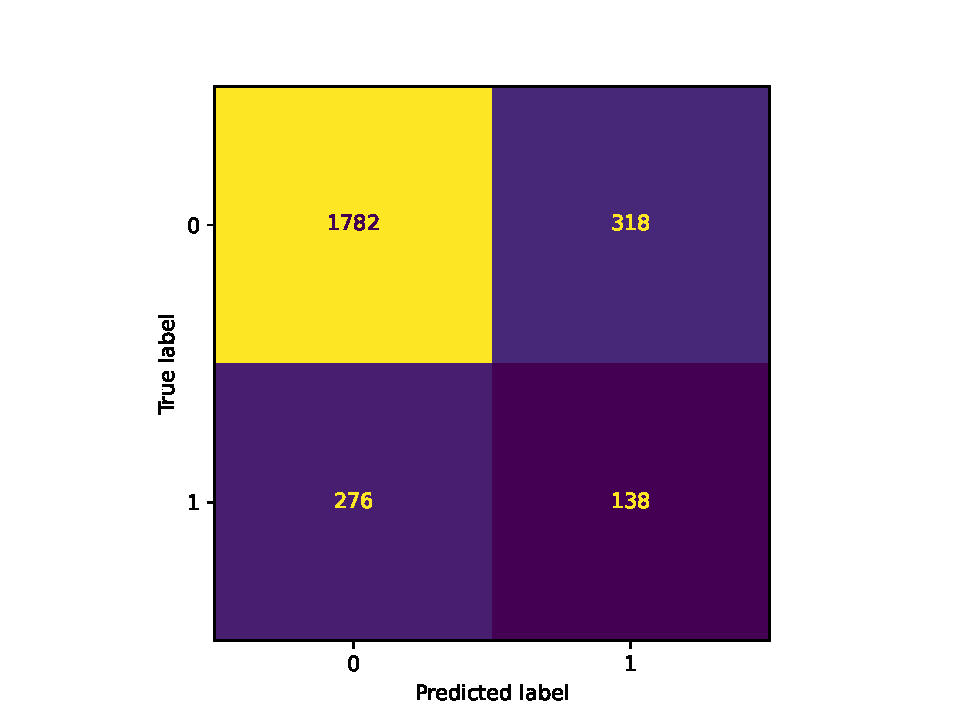
\includegraphics[width=\textwidth]{clf/holdout_confusion_matrix_.pdf}\caption{Holdout}\end{subfigure}
  \begin{subfigure}{0.43\textwidth}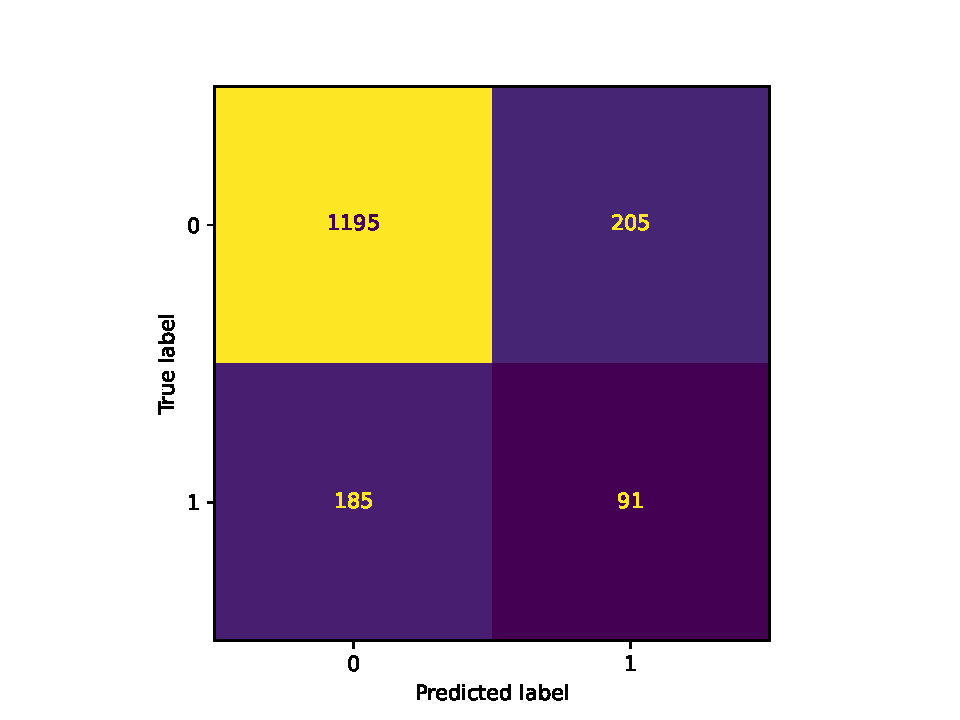
\includegraphics[width=\textwidth]{clf/cv_confusion_matrix_1.pdf}\caption{CV, partição 1}\end{subfigure}
  \begin{subfigure}{0.43\textwidth}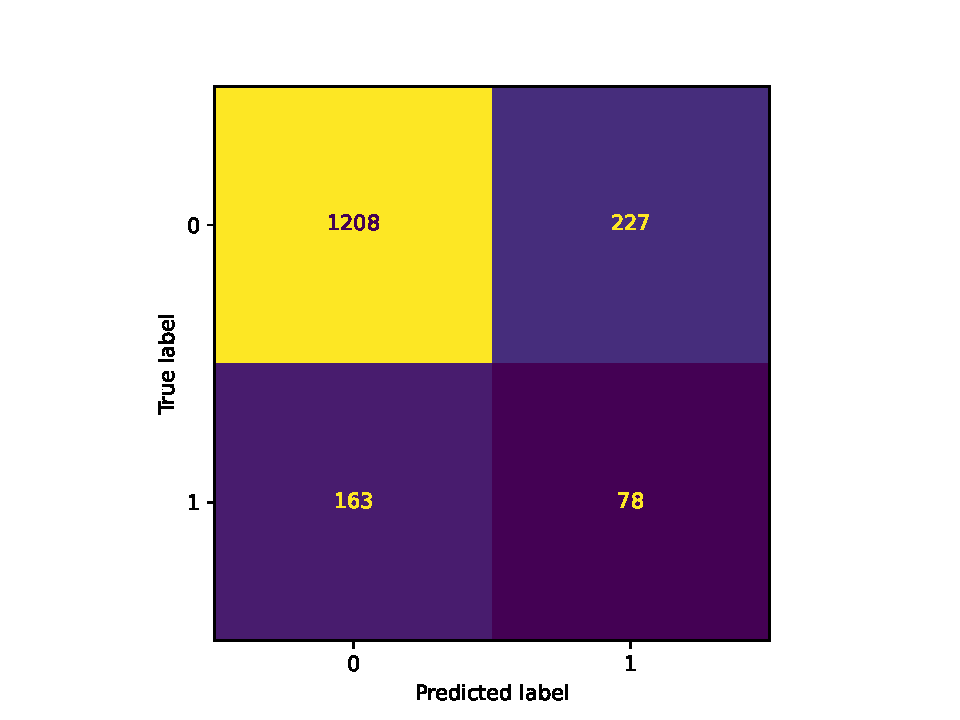
\includegraphics[width=\textwidth]{clf/cv_confusion_matrix_2.pdf}\caption{CV, partição 2}\end{subfigure}\\[0.5em]
  \begin{subfigure}{0.43\textwidth}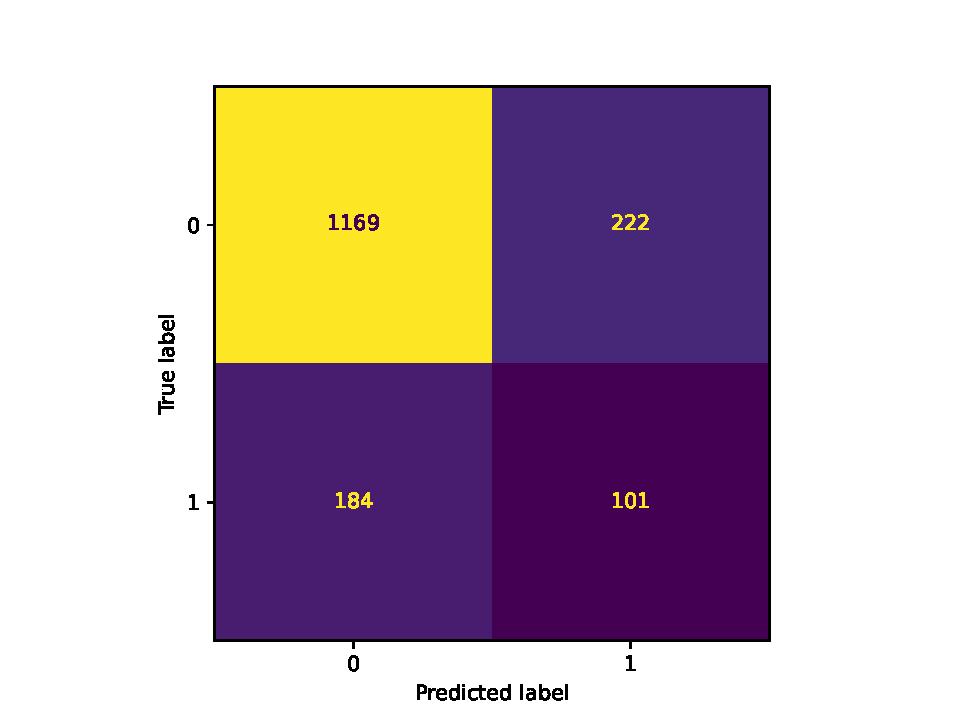
\includegraphics[width=\textwidth]{clf/cv_confusion_matrix_3.pdf}\caption{CV, partição 3}\end{subfigure}
  \begin{subfigure}{0.43\textwidth}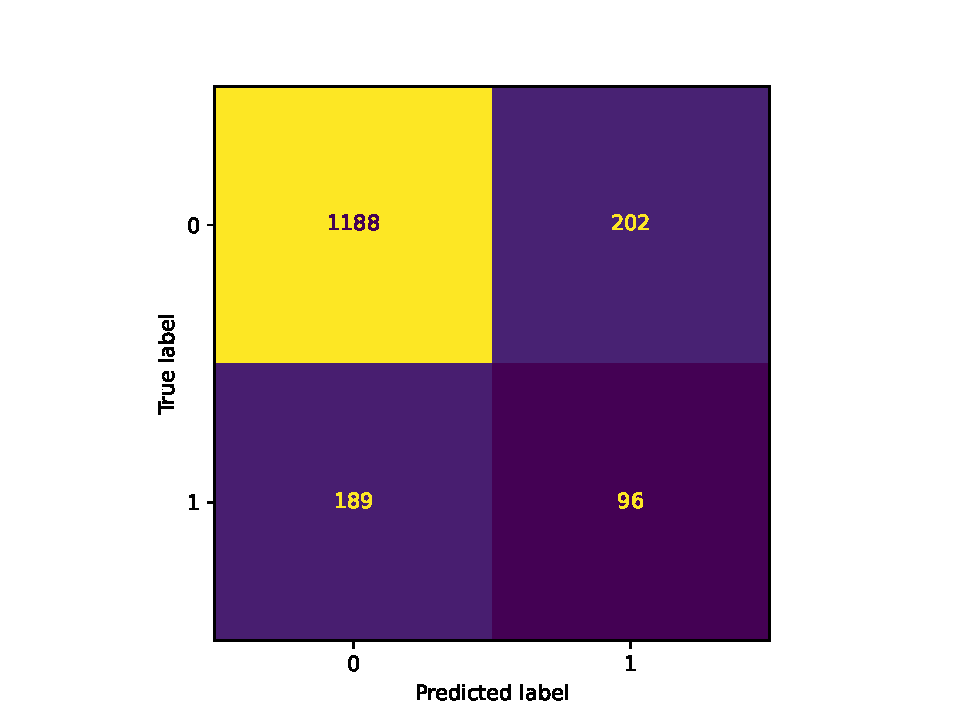
\includegraphics[width=\textwidth]{clf/cv_confusion_matrix_4.pdf}\caption{CV, partição 4}\end{subfigure}
  \begin{subfigure}{0.43\textwidth}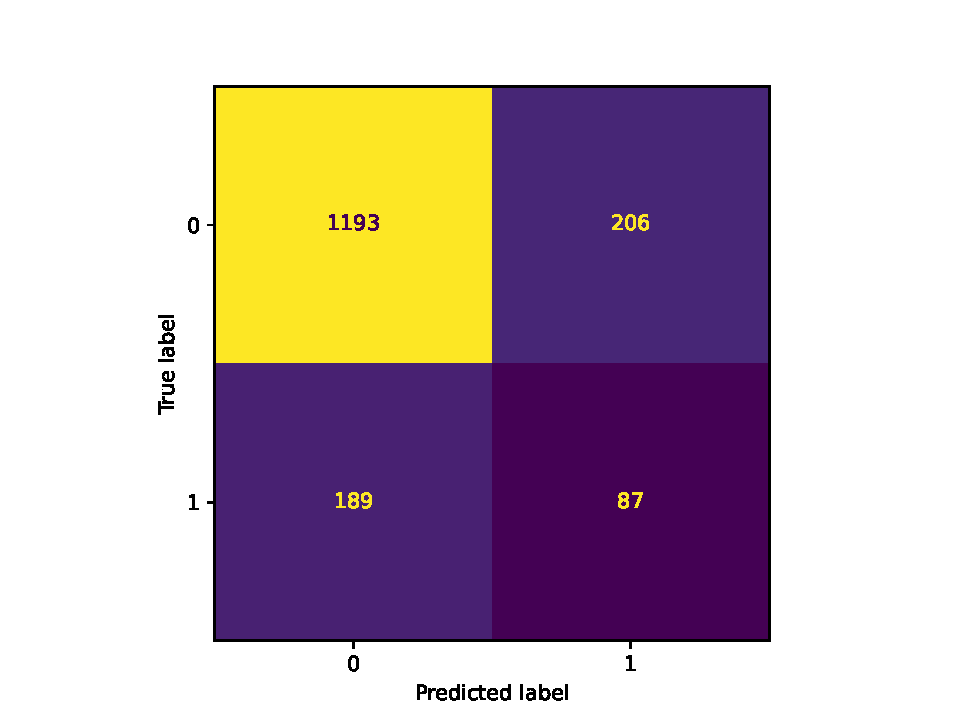
\includegraphics[width=\textwidth]{clf/cv_confusion_matrix_5.pdf}\caption{CV, partição 5}\end{subfigure}
  \caption{Matrizes de confusão da árvore de decisão (CART).}
  \label{fig:cart}
\end{figure}

\begin{figure}[H]
  \centering
  \begin{subfigure}{0.43\textwidth}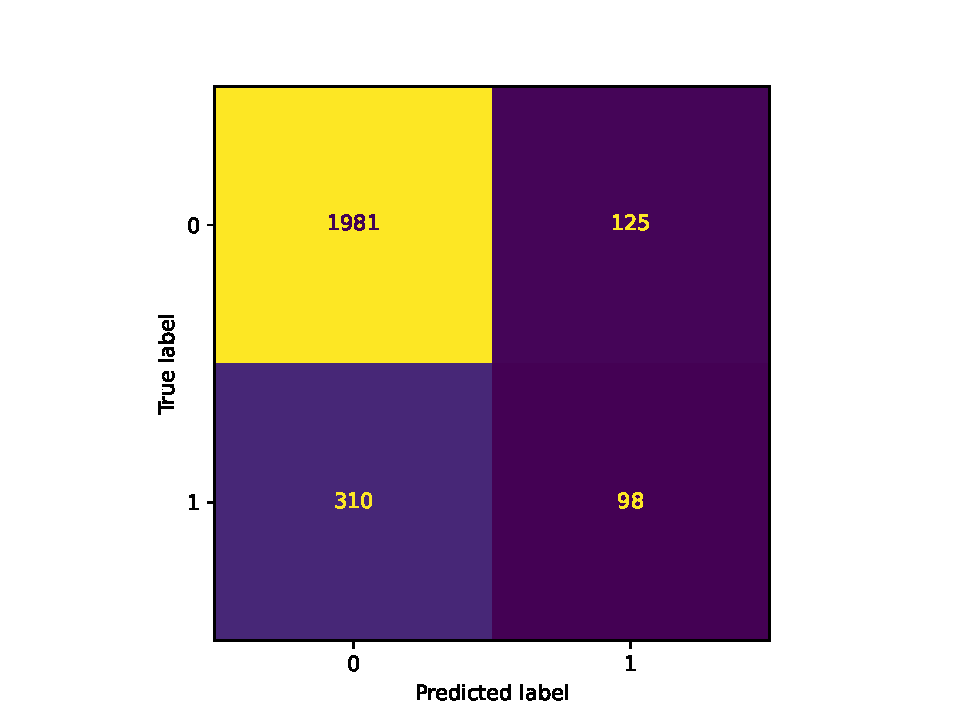
\includegraphics[width=\textwidth]{gnb/holdout_confusion_matrix_.pdf}\caption{Holdout}\end{subfigure}
  \begin{subfigure}{0.43\textwidth}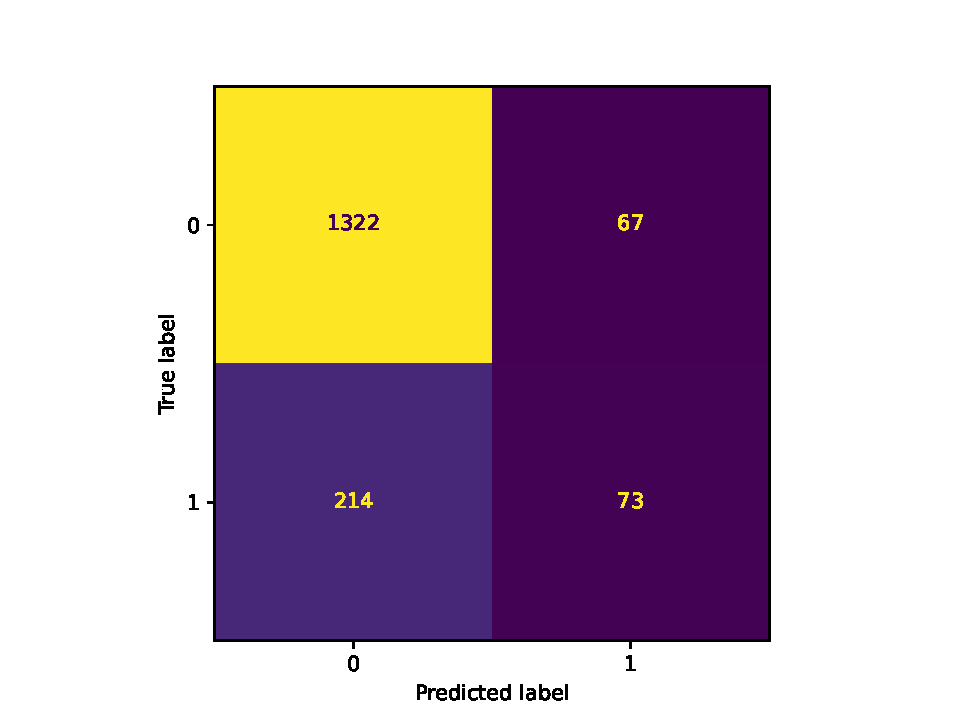
\includegraphics[width=\textwidth]{gnb/cv_confusion_matrix_1.pdf}\caption{CV, partição 1}\end{subfigure}
  \begin{subfigure}{0.43\textwidth}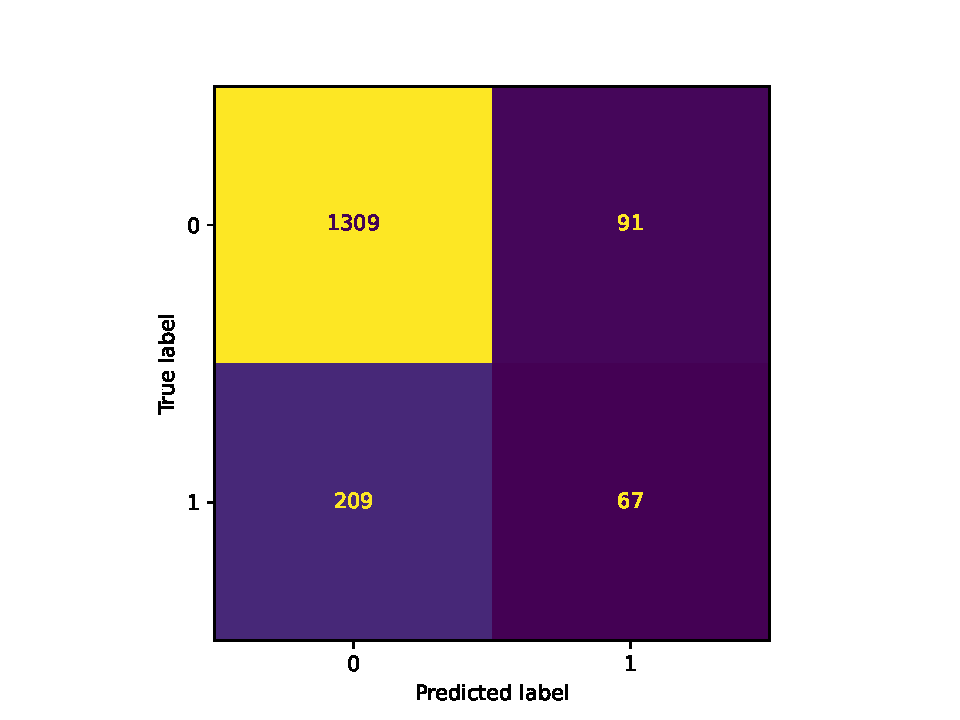
\includegraphics[width=\textwidth]{gnb/cv_confusion_matrix_2.pdf}\caption{CV, partição 2}\end{subfigure}\\[0.5em]
  \begin{subfigure}{0.43\textwidth}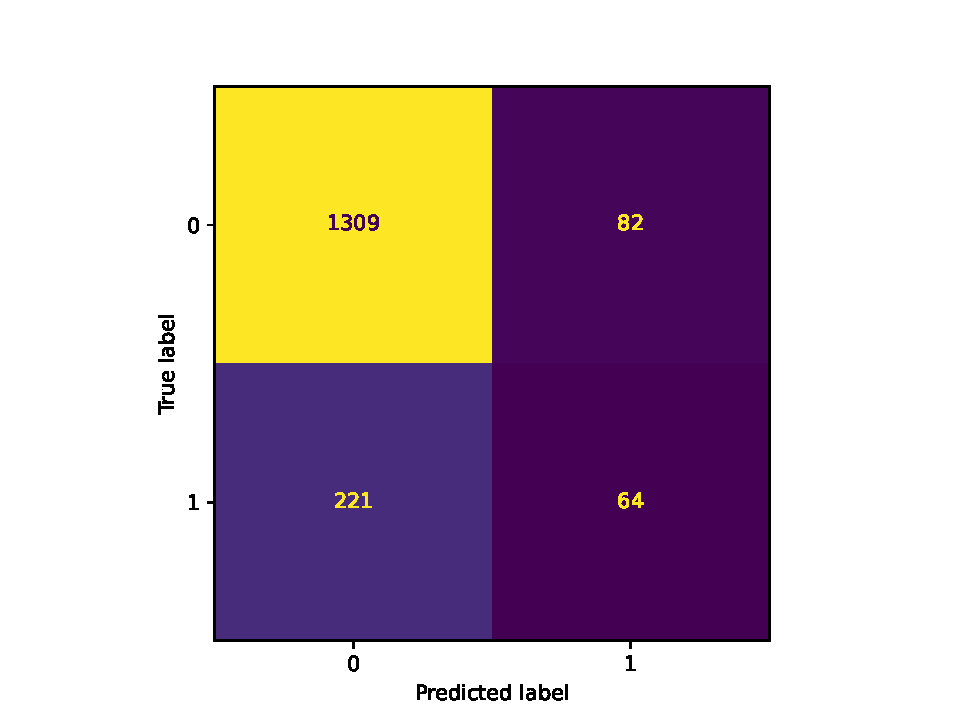
\includegraphics[width=\textwidth]{gnb/cv_confusion_matrix_3.pdf}\caption{CV, partição 3}\end{subfigure}
  \begin{subfigure}{0.43\textwidth}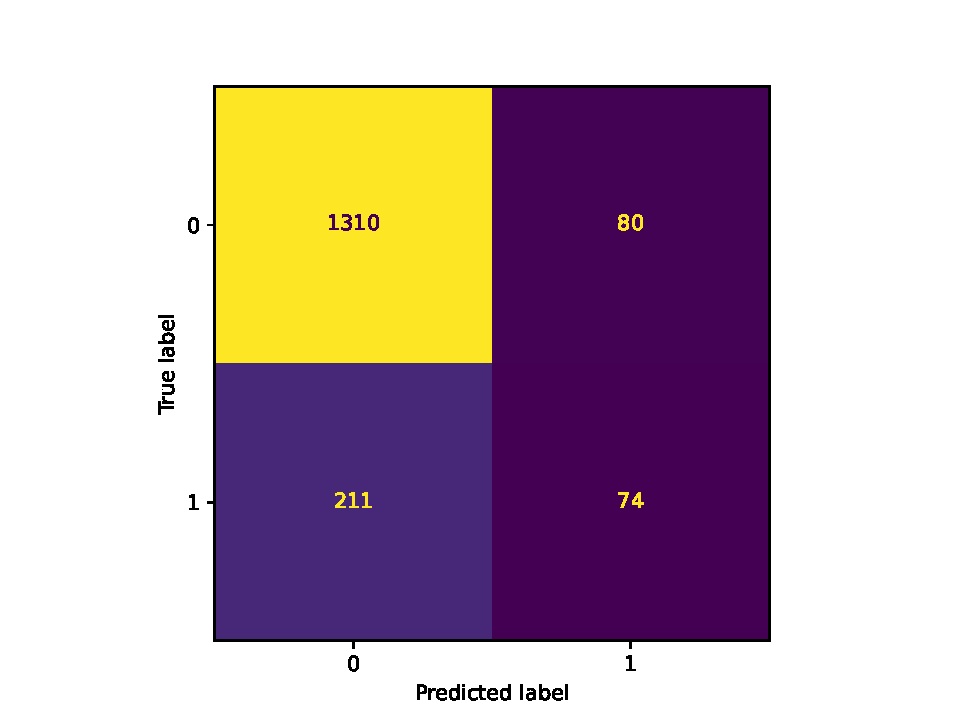
\includegraphics[width=\textwidth]{gnb/cv_confusion_matrix_4.pdf}\caption{CV, partição 4}\end{subfigure}
  \begin{subfigure}{0.43\textwidth}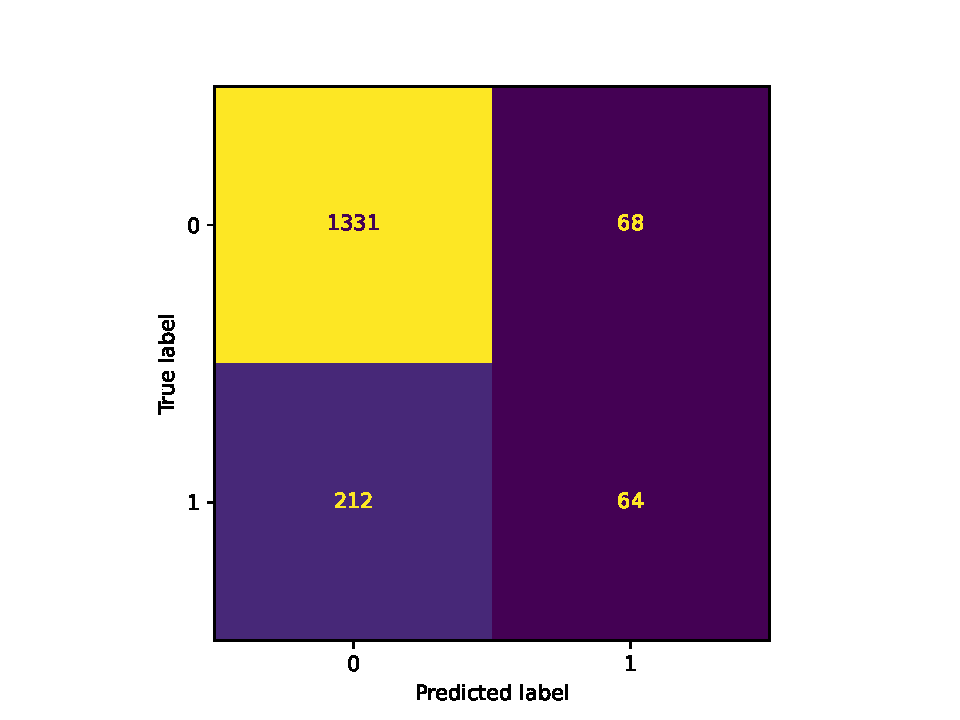
\includegraphics[width=\textwidth]{gnb/cv_confusion_matrix_5.pdf}\caption{CV, partição 5}\end{subfigure}
  \caption{Matrizes de confusão do Naive Bayes Gaussiano.}
  \label{fig:gnb}
\end{figure}

\subsection{Resultados}

A tabela~\ref{tab:res} resume as métricas obtidas.

\begin{table}[H]
  \centering
  \small
  \begin{tabular}{lcccc}
    \toprule
     & CART, holdout & CART, CV & Naive Bayes, holdout & Naive Bayes, CV \\
    \midrule
    Accuracy  & 0,765 & 0,766 & 0,827 & 0,827 \\
    Precision & 0,287 & 0,311 & 0,439 & 0,453 \\
    Recall    & 0,301 & 0,347 & 0,240 & 0,246 \\
    F1        & 0,294 & 0,328 & 0,311 & 0,319 \\
    \bottomrule
  \end{tabular}
  \caption{Métricas de desempenho (classe positiva: \code{match} = 1). CV: validação cruzada com 5 partições.}
  \label{tab:res}
\end{table}

As árvores de decisão resultantes são muito profundas. A figura~\ref{fig:arvores} mostra apenas os primeiros 6 níveis da árvore treinada em cada estratégia.

\begin{figure}[H]
  \centering
  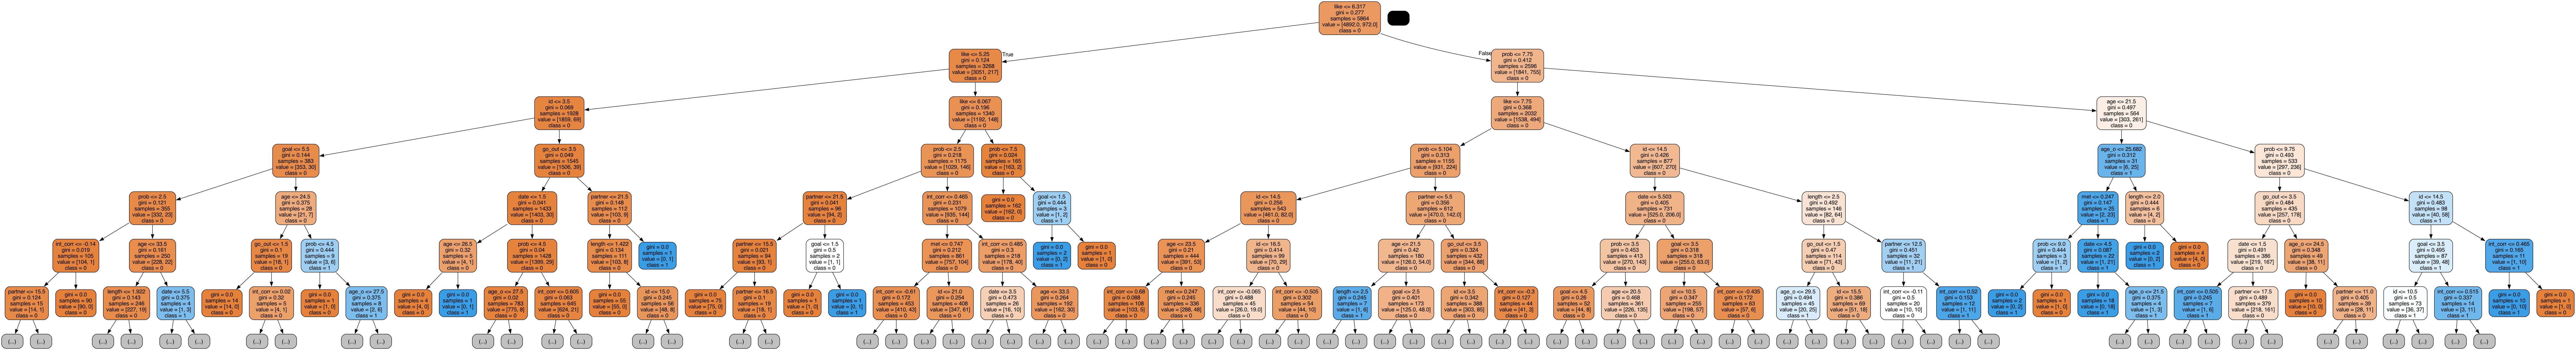
\includegraphics[width=\textwidth]{clf/holdout_tree_depth_6.png}\\[1em]
  
\includegraphics[width=\textwidth]{clf/cv_tree_depth_6.png}
  \caption{Primeiros 6 níveis da árvore de decisão: em cima, treinada no \emph{holdout}; em baixo, treinada na última partição da validação cruzada.}
  \label{fig:arvores}
\end{figure}

\subsection{Discussão crítica}

Com a \emph{accuracy}, nos quatro casos o modelo acerta em mais de três quartos dos casos, e o Naive Bayes é melhor (cerca de 0,83 contra 0,77). Esta métrica deve ser lida com cuidado: como 84\% dos exemplos são da classe 0, um classificador trivial teria \emph{accuracy} semelhante à do Naive Bayes. A \emph{accuracy} do CART, em particular, fica abaixo da de um classificador que prevê sempre 0.

A \emph{precision} mede, de todos os \emph{matches} previstos, quantos o são mesmo, ou seja, penaliza os falsos positivos. O Naive Bayes é claramente melhor (cerca de 0,44 a 0,45 contra 0,29 a 0,31): quando prevê \emph{match} acerta mais vezes. O \emph{recall} mede, de todos os \emph{matches} reais, quantos foram encontrados, ou seja, penaliza os falsos negativos. Aqui a árvore é melhor (0,30 e 0,35 contra 0,24 e 0,25): encontra mais \emph{matches}, ao custo de muitos falsos positivos. O Naive Bayes é mais conservador. O F1 combina as duas e é baixo em todos os casos (0,29 a 0,33), o que mostra que nenhum dos modelos prevê bem a classe minoritária. Os valores de F1 são próximos entre os dois algoritmos, pelo que não podemos dizer que um seja claramente melhor no geral.

Entre as duas estratégias de avaliação, a validação cruzada dá valores ligeiramente superiores em quase todas as métricas, mas as diferenças são pequenas (no máximo cerca de 0,05, no \emph{recall} da árvore). Com apenas uma execução de cada experiência e sem medir a variabilidade, não podemos concluir que esta diferença seja significativa.

\subsection{Limitações e dificuldades}
\label{sec:limitacoes}

\begin{itemize}
  \item \textbf{Desbalanceamento.} Só cerca de 16\% dos exemplos são positivos e não aplicámos nenhuma técnica de balanceamento (por exemplo, sobreamostragem da classe minoritária, subamostragem da maioritária ou pesos por classe), nem usámos validação cruzada estratificada. Isto prejudica o \emph{recall} e o F1.
  \item \textbf{Dimensão dos dados.} O conjunto tem pouco mais de oito mil exemplos e, na prática, muitos deles dizem respeito aos mesmos participantes. Com mais dados esperaríamos previsões melhores.
  \item \textbf{Identificador como atributo.} Usámos \code{id} (e \code{partner}) como atributos, embora sejam identificadores. Podem introduzir enviesamento, porque o mesmo participante aparece em várias linhas e o modelo pode aprender padrões específicos de cada pessoa. Não testámos o efeito de os retirar.
  \item \textbf{Substituição dos nulos antes da divisão.} Calculámos a média usando todos os dados, incluindo os de teste, antes de os dividir em treino e teste. O correto seria calcular a média só no conjunto de treino, para evitar fuga de informação. O efeito esperado é pequeno.
  \item \textbf{Árvore sem controlo de complexidade.} Não limitámos a profundidade nem podámos a árvore, pelo que há sobreajuste. Um valor de profundidade máxima escolhido por validação poderia melhorar a árvore.
  \item \textbf{Avaliação.} Cada experiência foi executada uma só vez, com sementes fixas, pelo que não medimos a variabilidade dos resultados. Também não otimizámos hiperparâmetros.
  \item \textbf{Dificuldades.} A principal dificuldade foi decidir como tratar os valores nulos sem perder demasiadas linhas, e perceber que a \emph{accuracy} era uma métrica enganadora neste problema. Surgiram ainda dificuldades práticas com a exportação das árvores, que exige o Graphviz instalado no sistema além da biblioteca Python.
\end{itemize}

\section{Conclusões}

Comparámos Árvores de Decisão (CART) e Naive Bayes Gaussiano na previsão de \emph{matches} em eventos de \emph{speed dating}, com \emph{holdout} e validação cruzada. O Naive Bayes tem melhor \emph{accuracy} (0,83 contra 0,77) e melhor \emph{precision}; a árvore tem melhor \emph{recall}. O F1 é baixo em todos os casos (0,29 a 0,33), porque a classe positiva é minoritária (cerca de 16\%) e a \emph{accuracy} sozinha é enganadora. A validação cruzada dá resultados ligeiramente melhores do que o \emph{holdout}, mas a diferença é pequena. A execução é muito rápida com estes dados e parâmetros. Como trabalho futuro, propomos balancear as classes, retirar os identificadores, calcular a média apenas no conjunto de treino e limitar a profundidade da árvore.

\begin{thebibliography}{9}
\bibitem{missing} \emph{A Comprehensive guide on handling Missing Values}. \url{https://medium.com/bycodegarage/a-comprehensive-guide-on-handling-missing-values-b1257a4866d1}\hfill\null
\bibitem{sklearn} Pedregosa \emph{et al.}, \emph{Scikit-learn: Machine Learning in Python}, Journal of Machine Learning Research, 12:2825--2830, 2011.
\bibitem{russell} S. Russell e P. Norvig, \emph{Artificial Intelligence: A Modern Approach}, Pearson, 4.ª ed., 2020.
\end{thebibliography}

\end{document}
